\chapter{MÉTODO DE VOLÚMENES FINITOS Y ESQUEMA DE ROE}
A continuación se describen el método y los esquemas a utilizar para llevar a cabo una solución numérica de una ecuación de conservación. La idea principal del capítulo es describir el método de volúmenes finitos y la motivación de su uso. Se explicarán los esquemas adecuados para aplicar el mencionado método, un solucionador del problema de Riemann, denominado esquema de Godunov y otro solucionador aproximado del problema de Riemann, denominado esquema de Roe. Este último es el esquema elegido para resolver las ecuaciones de Euler en este texto.\\
El contenido de este capítulo se basa en la parte \textit{Numerical Methods} del texto \cite{Leveque} de Randall LeVeque.

\section{Método de volúmenes finitos}
El método de volúmenes finitos (MVF) es un método numérico de integración que se especializa en resolver ecuaciones diferenciales escritas en forma conservativa. El MVF destaca por ofrecer una interpretación peculiar de la función a resolver, ya que es un método basado en la forma \textbf{integral} de las ecuaciones.
\subsection{Discretización del problema}
Al aplicar un método numérico para resolver una ecuación diferencial se necesita discretizar el dominio de la función y la función misma, redefiniendo algunas nociones matemáticas y utilizando aproximaciones. Sea  $D = [a,b]$ el dominio espacial de la solución de una ecuación de conservación. Para aplicar el MVF, este dominio se divide en $N$ intervalos iguales llamados \textbf{celdas}. Cada celda se denomina $\mathcal{C}_i$ y se define como un intervalo, $\mathcal{C}_i = [x_i, x_{i+1}]$. Además, cada celta tiene un ancho $h$ \footnote{La diferencia entre dos puntos sobre el eje $x$ también se denomina $\Delta x$, pero se opta por usar $h$ como símbolo, para evitar escribir ecuaciones engorrosas.}, dado por
\begin{equation}
	h = \frac{b-a}{N}.
\end{equation}
Por lo tanto, se tiene una expresión para el valor de cada $x_i$,
\begin{equation}
	x_i = a + (i-1)h.
\end{equation} 
\begin{figure}[ht]
	\centering
	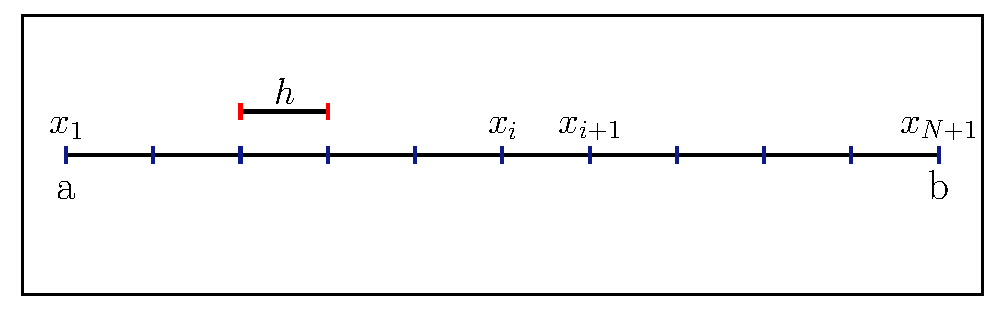
\includegraphics[width=\linewidth]{../some_plots/cap2/graficas/domain.pdf}
	\label{fig:discretizacion-eje-x}
	\caption{Esquema de símbolos utilizados para la discretización del dominio espacial. \textbf{Fuente:} elaboración propia.}
\end{figure}
El dominio temporal, dado por la variable $t$, se discretiza de forma similar. El instante inicial $t_0$ corresponde a $t=0$, de tal manera que cada instante consecuente está separado por un múltiplo entero de una cantidad $k$ denominada \textit{salto temporal}. Por lo tanto, el enésimo instante de tiempo queda como
\begin{equation}
	t_n = nk, \hspace{1cm} \forall n \in \mathbb{N}.
\end{equation}
Para referirse a la función $\mathbf{U}$ discretizada se utilizará una notación especial, esta es,
\begin{equation}
	\mathbf{U}(x_i, t_n) \approx U_{i}^{n}
\end{equation}
que se interpreta como el valor aproximado numéricamente de la función $\mathbf{U}$ en el punto $(x_i, t_n)$. Para conseguir dicha aproximación, el MVF utiliza la siguiente expresión
\begin{equation}
	U_{i}^{n} \approx \frac{1}{h}\int_{x_i}^{x_{i+1}}\mathbf{U}(x, t_n)\dd{x} \equiv \frac{1}{h}\int_{\mathcal{C}_i}\mathbf{U}(x, t_n)\dd{x}
\end{equation}
de tal manera que, aproximadamente, $U_i^n$ toma el valor promedio de $\mathbf{U}(x,t_n)$ sobre la celda $\mathcal{C}_i$. Vale la pena destacar que si las funciones $u_j$ de las que depende $\mathbf{U}$ son funciones suaves, la expresión para $U_i^n$ coincide en $\mathcal{O}(h^2)$ con el valor exacto de $\mathbf{U}$ en el punto medio de la i-ésima celda.

La ventaja de utilizar un método aproximado basado en los valores promedio de las funciones en las celdas es que este puede considerarse un método \textbf{conservativo} de tal manera que imite la ley de conservación obtenida a partir de la forma integral de la ecuación de conservación. Esta ventaja es sumamente importante al considerar ondas de choque como posibles soluciones.
